\documentclass{ReportTemplate}
\usepackage{titlesec}
\usepackage[francais]{babel}
\usepackage[T1]{fontenc}
\title{CSEL}
\author{Macherel Rémy}
\date{\today}
\subtitle{Rapports des TP}
\subsubtitle{Git du projet : \href{https://github.com/Mathistis/csel-workspace}{https://github.com/Mathistis/csel-workspace}}
\location{Fribourg,}
\contact{remy.macherel@master.hes-so.ch}
\version{1.0}
\titlespacing*{\chapter}{0pt}{-60pt}{20pt}
\begin{document}

\maketitlepage

\newpage

\maketableofcontent

\medskip

\titleformat{\chapter}[display]
    {\Huge\bfseries}
    {}
    {0pt}
    {\thechapter.\ }
    

\chapter{Introduction}
Ce rapport décrit l'architecture ainsi que le développement et les
fonctionnalités du mini-projet réalisé lors du cours \textit{MA-CSEL} suivi lors
du semestre de printemps 2022 du master MSE. Ce projet consiste à mettre en
pratique les notions vues dans le cours par l'intermédiaire de l'implémentation
d'un gestionnaire de ventilateur pour le processeur de la cible. Notre cible
n'ayant pas de réel ventilateur, son fonctionnement sera simulé par le
clignotement d'une LED symbolisant la fréquence de celui-ci ainsi qu'un écran
OLED affichant quelques valeurs importantes.\newline
Le but du travail est donc de concevoir une application permettant de simuler la
gestion de la vitesse de rotation d'un ventilateur en fonction de la température
du processeur. Les fonctionnalités suivantes seront donc implémentées:
\begin{itemize}
    \item Supervision de la température du processeur et la gestion de la
    vitesse de clignotement de la LED à l'aide d'un module noyau.
    \item Un daemon en espace utilisateur qui offrira des services pour une
    gestion manuelle et prendra en compte la gestion des appuis sur les boutons
    afin d'augmenter la vitesse de rotation, de la diminuer et de passer du mode
    manuel à automatique.\newline
    Ce daemon pourra également, à l'aide d'une interface IPC, communiquer avec
    une application de type \textit{CLI} pour la gestion du clignotement et du
    mode.
    \item Une application \textit{CLI} pour piloter le système via l'interface IPC.
\end{itemize}

\chapter{Architecture logicielle}
\begin{figure}[H]
    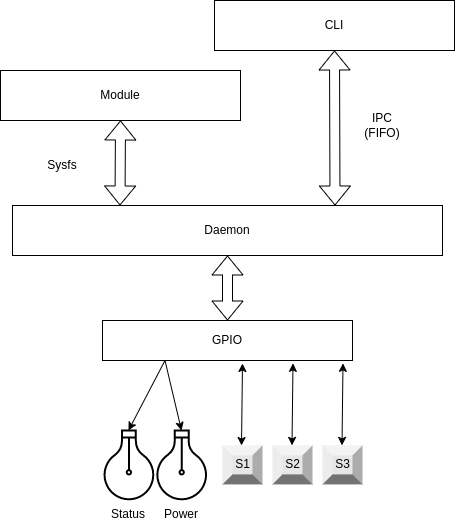
\includegraphics[width= \textwidth]{imageSources/Diagramme_Fonctions.drawio.png}
    \caption{Diagramme de principe de l'application}
    \label{fig:functionDiagram}
\end{figure}

\chapter{Conception du daemon}
Ce chapitre traite du développement du deamon offrant les services permettant la
gestion de la fréquence ainsi que le choix du mode.

\end{document}


